\documentclass[openright,twoside,headsepline]{scrbook}
\usepackage{graphicx,color,scrpage2}
\definecolor{Cayenne}{rgb}{0.502,0.0,0.0}
\definecolor{Steel}{rgb}{0.4,0.4,0.4}

\addtokomafont{chapter}{\color{Steel}}
\addtokomafont{section}{\color{Steel}}
\addtokomafont{subsection}{\color{Steel}}
\addtokomafont{subsubsection}{\color{Steel}}
\addtokomafont{paragraph}{\color{Steel}}
\addtokomafont{pagehead}{\color{Steel}}
\renewcommand{\pnumfont}{\color{Steel}} 
\addtokomafont{headsepline}{\color{Steel}} 
\pagestyle{scrheadings} 

\usepackage[applemac]{inputenc}
\usepackage{amsmath,amssymb,amsfonts,amsthm}
\usepackage[leftcaption]{sidecap} % inner, outer,left,right
\sidecaptionvpos{figure}{t}


\usepackage[format=plain,singlelinecheck=false, font={sf,small},labelfont={bf,color=Steel}]{caption}
\DeclareCaptionLabelSeparator{cayenne_period}{\textcolor{Cayenne}{.} }
\captionsetup{labelsep=cayenne_period}

\begin{document}
\graphicspath{{/Users/lentz/Documents/GitHub_locals/Thesis/images/}}

\chapter{Theory}
This chapter is devoted to the mathematical formalism that is used to model infectious diseases and networks.
The author defines a mathematical framework and summarizes relevant results of earlier research in this area.
In addition, section xx describes an efficient computer implementation of networks.

\section{Models of infectious diseases}
%\subsection{Very briefly:}
\paragraph{Observations\color{Cayenne}{.}} Large scale patterns of epidemics have been measured \cite{giehl:2012}.
The spread of infectious diseases is something that everyone is familiar with.

\paragraph{Research field: Epidemiology\color{Cayenne}{.}} One goal of epidemiology is to understand the principles behind the spreading process, i.e. the way how a disease is transmitted through a population.
In this context, \emph{conceptional} models are used.
They make use of simple assumptions for the local (person-to-person) dynamics and focus on the big picture of the process.
Conceptual models are very similar to models in theoretical physics, because they focus on the very essence of the problem (here: the macroscopic view, spreading patterns).
However, they have to neglect many details of the real problem (here: physiology, symptoms, individual behavior, infection pathways and many more!) in order to have mathematical feasible models.

Another important issue of epidemiology is the \emph{forecast} of epidemic spreading processes.
Forecast models incorporate as much information as possible and the main focus is not an understanding of the basic principles.

This section summarizes the mathematical framework that roughly reproduces the behavior of infectious diseases and briefly discusses some major insights.


\subsection{Development of mathematical epidemiology}
The modeling of infection diseases mostly uses the concept of compartment models as explained in section xx.
Major contributions to the modern theoretical framework were provided by \cite{kermack:27}, \cite{bailey:57} and \cite{andersonmay:92}.
In his review about the mathematics of infectious diseases Hethcote reports a model for smallpox was already formulated in 1760 by D. Bernoulli (\cite{Hethcote:2000} and references therein).
In the early 20th century, people developed mathematical models for epidemics: a discrete time model in 1906 \cite{Hamer} and a differential equation model in 1911 \cite{Ross}.
The epidemic threshold (section \ref{sec:sir_model}) was found in the 1920s \cite{kermack:1927_thresh} \cite{kermack:27}.
Starting from Bailey's book \cite{bailey:57} in the 1950s, the modeling of infectious diseases became a major scientific research field.
Modern models of infectious diseases include vaccination, demographic structure, disease vectors, quarantine and even game theory (\cite{Bauch:2004} and references in \cite{Hethcote:2000}).
The availability of contact data in recent years led to a strong impact on network analysis on epidemiology.
Well known concepts of mathematics (graph theory \cite{Bollobas:1985}) and social sciences (social network analysis \cite{WassermanFaust}) have been adopted to disease modeling, since the connections between individuals are related to their epidemic spreading potential \cite{Keeling:2005}.

\subsection{Infection dynamics}

The spread of infectious diseases can be modeled in terms of compartment models as described in section xx.
We differentiate between \emph{conceptional models} and \emph{realistic disease models}.
While the former class is used to provide conceptual results as for the computation of thresholds or to test theories \cite{Hethcote:2000}, realistic disease models use as many aspects as possible to provide a forecast of the spreading process.
Realistic disease models can be very complex and are beyond the scope of this work, thus the author focuses on the use of conceptional models.
The following section is inspired by the Lecture notes of J.~R.~Chasnov \cite{Chasnov:2010}.

\subsection{SI model}\label{sec:si_model}
Let us consider a population of $N$ individuals.
In the simplest case, the infection status of each individual is either susceptible or infected and there are no births and deaths on the population.
Susceptible individuals become infected, if they are in contact with an infected.
This mimics the behavior of an infectious disease without immunization, i.e. infected individuals stay permanently infected.

Provided that $\alpha $ is the rate, under which new susceptible become infected, the SI-model is as follows:
\begin{align}\label{eq:si_model}
\frac{dS}{dt} &= -\alpha SI \nonumber \\
\frac{dI}{dt} &= \alpha SI,
\end{align}
where $S$ and $I$ are the numbers of susceptible and infected individuals respectively.
The total population is $N=S+I$.
Thus, \eqref{eq:si_model} can be rewritten as
\[
\frac{dI}{dt}=\alpha (N-I)I,
\]
i.e. a logistic differential equation.
Hence, in the limit $t\rightarrow \infty $ the whole population is infected ($I(\infty )=N$). 

\subsection{SIR model}\label{sec:sir_model}
In contrast of the infection dynamics introduced in the previous section, many epidemics allow for an immunization of the individuals.
Examples are measles or whooping cough \cite{grenfell:92} \cite{andersonmay:92}.
In this case, individuals recover from the disease after being infected for a certain time period.
The infection scheme has to be extended to susceptible-infected-recovered (SIR) as in the following infection model \cite{kermack:27}:
\begin{align}\label{eq:sir_model}
\frac{dS}{dt} &= -\alpha SI \nonumber \\
\frac{dI}{dt} &= \alpha SI -\gamma I \nonumber \\
\frac{dR}{dt} &= \gamma I
\end{align}
where $\alpha $ is the infection rate and $\gamma $ is the immunization or recovery rate.
There is no analytic solution for the system \eqref{eq:sir_model}, but some fundamental conclusions can be obtained analytically.
We show a typical solution of \eqref{eq:sir_model} in figure \ref{fig:std_sir_model}.
%
\begin{SCfigure}%[htbp]
%\begin{center}
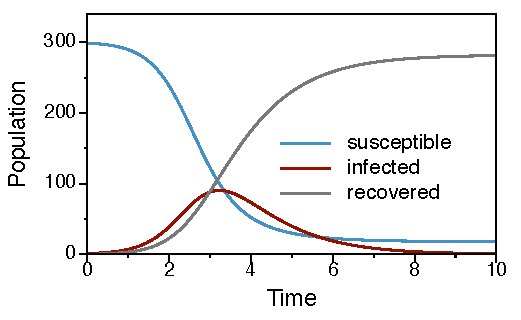
\includegraphics{sir_model.pdf}
\caption{Solution of the susceptible-infected-recovered (SIR) model \eqref{eq:sir_model}.
The number of infected shows that the spreading process is a single event.
Note that a fraction of the population is still susceptible at the end of the process.
Parameters: $\alpha = 3$, $\gamma = 1$, $N=300$, $S_0=1$.}
\label{fig:std_sir_model}
%\end{center}
\end{SCfigure}
%


The SIR model shows more sophisticated features than the SI model \eqref{eq:si_model}.
To begin with, we analyze the fixed points of the system, i.e. $(S_*,I_*,R_*)$ where
\begin{equation}
\frac{dS_*}{dt} = -\alpha S_*I_* =0 ,\; \;\;
\frac{dI_*}{dt} = \alpha S_*I_* -\gamma I_* =0,\; \;\;
\frac{dR_*}{dt} = \gamma I_* = 0.
\end{equation}
It follows from the last equation that $I_*=0$ at the fixed point, where $S_*$ and $R_*$ can be arbitrary.
Hence, a fixed point is $(S_*,0,R_*)$.

Let us analyze the stability of the fixed point in the early phase of an infection.
Almost all individuals are susceptible and consequently $I_*=N-S_*$.
An outbreak occurs, if and only if $dI/dt >0$ in this phase, i.e.
\begin{equation}\label{eq:prelim_condition}
\frac{dI}{dt}=\alpha S_* (N-S_*) - \gamma (N-S_*)=(N-S_*)(\alpha S_* -\gamma ) >0.
\end{equation}
It follows from \eqref{eq:prelim_condition} that the number of infected grows, if
\begin{equation}\label{eq:prelim_rnod}
\alpha S_* / \gamma >1.
\end{equation}
Equation \eqref{eq:prelim_rnod} is extremely important in epidemiology, because it defines a threshold for the unfolding of an infection spreading process.
We call this fraction the \emph{basic reproduction number} $R_0$.
Recall that $S_* \approx N$ in the fixed point.
Thus it follows that the outbreak condition is
\begin{equation} \label{eq:r0}
R_0 = N \frac{\alpha }{\gamma } >1.
\end{equation}

The basic reproduction number describes the average number of follow-up infections by each infected individual.
It is one of the main goals in epidemiology to bring down the basic reproduction number of a disease below the critical value $R_0=1$.
This is the reason for the implementation of mass vaccination.
As one can immediately see from equation \eqref{eq:r0}, this can be done by reducing the infection rate $\alpha $ or by increasing the immunization rate $\gamma $.
In principle, one could also reduce the size of the initial population $S_*$.
As an example, reducing the infection rate can be done by increasing hygiene standards or appropriate behavior, say wearing warm clothes in winter time to avoid common cold.
The immunization rate can be increased by vaccination.

Let us now focus on the late phase of an SIR-infection.
In contrast to the SI-model of section \ref{sec:si_model} an SIR like outbreak does not necessarily infect the whole population, even if $R_0>1$.
The reason is that there has to be a critical mass of susceptible individuals in order to keep an infection alive (see equation \eqref{eq:prelim_rnod}).
The total number of infected during an infection given by the number of recovered at the end of the infection, since every recovered has to be in the infected state in the first place.
A central measure throughout this work is therefore the \emph{outbreak size} $R_\infty$.

To compute the outbreak size, we consider the second fixed point of \eqref{eq:sir_model}, i.e. the fixed point for $t \rightarrow \infty $.
At this point there are no infected and a fraction of the population is recovered.
Hence the fixed point is $(N-R_\infty , 0, R_\infty )$.
A simple way to obtain the outbreak size $R_\infty $ is to use equations \eqref{eq:sir_model} and compute 
\[
\frac{dS}{dR}=-\frac{\alpha }{\gamma } S 
\]
and separate the variables \cite{Chasnov:2010}.
This yields
\[
\int _{S_*} ^{N-R_\infty} \frac{dS}{S}=-\frac{\alpha }{\gamma } \int _{R_*} ^{R_\infty} dR .
\]
We integrate from the initial condition at $t=0$ to the final condition at $t \rightarrow \infty$, where $S_\infty = N-R_\infty $.
Using that $R_* =0$ at $t=0$ gives 
\begin{equation}\label{eq:transcendental}
R_\infty = S_*-S_* e ^{-\frac{\alpha}{\gamma}R_\infty}.
\end{equation}
This transcendental equation can be solved numerically using a Newton-Raphson technique.
The outbreak size $R_\infty $ only takes finite values for $\alpha / \gamma > 1$.
A solution of equation \eqref{eq:transcendental} is shown in figure \ref{fig:transcendental}
%
\begin{figure}[htbp]
\begin{center}
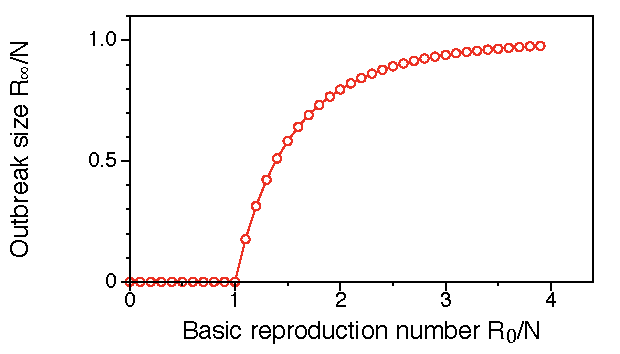
\includegraphics{R_0_R_infty.pdf}
\caption{Relative outbreak size vs. basic reproduction number.
The outbreak size takes finite values only for $R_0/N >1$.
Note that even for supercritical $R_0$ the outbreak size is in general smaller than the total population.
}
\label{fig:transcendental}
\end{center}
\end{figure}

It should be noted that an SIR epidemic is a single event, i.e. it possesses a \emph{characteristic time scale}.
The analysis of the late phase of an epidemic also gives information about these time scales.
Let us consider the second equation of \eqref{eq:sir_model}.
\begin{equation}\label{eq:sir_model_only_i}
\frac{dI}{dt} = \alpha SI -\gamma I
\end{equation}
In the late phase of an SIR-type epidemic, the fraction of infected is small.
Given sufficiently large values of $R_0$, the fraction of recovered is also small in this phase (see figure \ref{fig:transcendental}).
Thus, we neglect the quadratic term in \eqref{eq:sir_model_only_i}.
This gives $\frac{dI}{dt} = -\gamma I $, which has the solution
\[
I(t)=I(0)e^{-\gamma t}.
\]
Hence, the infection decays exponentially for large $t$ and the inverse recovery rate $1/\gamma $ defines the characteristic time of the epidemic.

\subsection{Force of infection}
The model presented in section \ref{sec:sir_model} describes only the very basic behavior of epidemic dynamics, and is therefore a conceptual model.
However, it is one of the main objectives in epidemiology to have an understanding of the exact infection rates in the process.
Infection rates their selves can cause complex infection dynamics.

The term $\alpha I$ used in section \ref{sec:sir_model} is a special, very simple case of an infection rate.
More generally, we have to replace $\alpha I$ by an abstract infection rate $\lambda $ containing more information about the interaction between susceptible and infected individuals \cite{Keeling:2005}.
Thus, the equation for the infected becomes
\[
dI/dt = -\lambda S -\gamma I.
\]
The rate $\lambda $ is called the \emph{force of infection}.
In principle, this parameter can be arbitrarily complex, because it contains detailed information about the mixing properties of the population.
This information could be given as contact networks, demographic contact structures, etc.

In most cases, detailed information about mixing is not available.
Instead, we assume \emph{random mixing} of the population, i.e. every individual can be in contact with every other individual.
This yields a transmission rate \cite{Keeling:2005}
\begin{equation}\label{eq:force_of_infection}
\lambda = \tau n \frac{I}{N}\equiv \beta \frac{I}{N},
\end{equation}
where $\tau $ is the transmission rate, $n$ is the effective contact rate and $I/N$ is the fraction of infectious contacts.
It is therefore reasonable to replace the infection term $\alpha $ in \eqref{eq:sir_model} by $\beta /N$ to explicitly include the force of infection.
Nevertheless, the results presented in section \ref{sec:sir_model} remain qualitatively the same.

Although the force of infection gives a more reasonable description of the infection process, the assumption of random mixing remains inappropriate for many real world systems.
Due to the availability of contact data, the random mixing assumption can be improved in terms of contact networks.
Even if the exact data of an epidemic system is not available, research on complex networks allows us to give more realistic models about mixing.
In the next section, we briefly report important results in complex network research and focus on the interplay between networks and epidemics in section xx.


\section{Network theory}
As we have seen in the previous section, standard epidemic models make use of the random mixing assumption.
This assumption seems reasonable, if no further information about the contact structure within a population is available, because it gives a worst case scenario of the infection dynamics.
Even an overestimation of the outbreak size can be corrected by introducing smaller, effective disease parameters.
However, the random mixing assumption does not allow for non homogenous mixing, i.e. each individual is considered equal.
Nevertheless, the equality of individuals is not a reasonable assumption for many epidemic substrates.
Examples are contact structures of humans, livestock trade, vehicles as disease vectors of links between computers.

\subsection{Network matrix representations}\label{sec:network_matrices}
A network is a system consisting of nodes that are connected by edges.
Edges can be undirected, directed and weighted.
In principle, a network can consist of edges of different types.
This can be represented by multiple networks sharing the same set of nodes, but different edges.

Networks are called graphs in mathematical literature.
A graph $G=(V,E)$ is a set of nodes (or vertices) $V$ and edges (or arcs) $E$, where each edge is given by the tuple of nodes it connects, i.e. $e_1 =(u,v) \in E$ connects nodes $u$ and $v$.
An edge $(u,v)$ being present in an undirected network implies an edge $(v,u)$.
Apparently, this does not hold in directed networks.
Edges of weighted networks carry additional meta information about their weight.
This meta information can be their importance, capacity, number of transported items or the geographical distance between nodes $u$ and $v$.

Graphs can be represented by different graph matrices, where different matrix representation emphasize typical properties of the network.
The most common graph matrix is the \emph{adjacency matrix} $\mathbf{A}$ with entries
\begin{equation}\label{eq:adjacency_matrix}
a_{ij}\equiv (\mathbf{A})_{ij}= 
\begin{cases}
1 & \text{if $i$ is connected to $j$} \\
0 & \text{else.}
\end{cases} 
\end{equation}
An adjacency matrix contains the edges of the graph and can be seen of the most fundamental graph representation.
Figure \ref{fig:simple_digraph} shows a simple example of a directed graph and its adjacency matrix.
The corresponding matrix would be symmetric in the undirected case.
Weighted networks can be represented by weight matrices, where the values of the entries in \eqref{eq:adjacency_matrix} are not restricted to zero and one.
%
\begin{SCfigure}%[h]
%\begin{center}
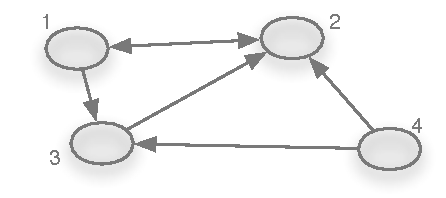
\includegraphics{Simple_DiGraph}
\caption[Adjacency matrix.]{A simple directed network. The corresponding adjacency matrix is
\[
\mathbf{A}=\left(\begin{array}{cccc}0 & 1 & 1 & 0 \\1 & 0 & 0 & 0 \\0 & 1 & 0 & 0 \\0 & 1 & 1 & 0\end{array}\right).
\]
}
\label{fig:simple_digraph}
%\end{center}
\end{SCfigure}

The adjacency matrix of an undirected network is symmetric, because every non-zero entry $a_{ij}=1$ implies an edge into the opposite direction, $a_{ji}=1$.
Entries on the main diagonal $a_{ii}$ correspond to nodes with self loops, i.e. nodes with edges pointing back to themselves.
The $i$-th row the adjacency matrix contains non-zero entries $a_{ij}=1$, whenever node $i$ is connected to node $j$.
Hence, every row can be interpreted as the neighborhood of one node.
This holds for undirected and for directed networks.
The columns of $\mathbf{A}$ give the same information as the rows.
In the directed case, however, rows contain the out-neighborhood of each node and columns contain the in-neighborhood, respectively.

A Markov chain is a random process without memory and with discrete state space and discrete time.
It is called time-homogenous, if the transition rates are constant.
Time-homogenous Markov chains can be represented as weighted networks and the corresponding weighted adjacency matrix is the \emph{transition matrix}.
Transition matrices are stochastic matrices, i.e. the elements of every row sum up to unity.
Each node represents a different state of the system and the edges are weighted with the probabilities to transition into other states adjacent to these edges.
It is obvious that a transition matrix representation is useful to describe random walks on networks.
An example of such a process is shown in figure \ref{fig:markov_chain}.
The underlying network represents a line of locations, where the drunkard can be located.
At every time-step there is a certain probability to move to another location.
%
\begin{SCfigure}%[htbp]
%\begin{center}
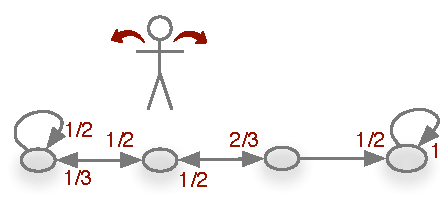
\includegraphics{Markov_chain.pdf}
\caption{Trajectory of a toddling drunk man as an example of a Markov chain.
At every location there is a probability for the drunkard to go left or right.
The node rightmost node is an absorbing state and could model a park bench.
Weights at arrowheads mark the transition probability.
(inspired by \cite{Aldous_book}).}
\label{fig:markov_chain}
%\end{center}
\end{SCfigure}
%
The state of the random walker can be described by a probability vector $\mathbf{p}$, where the initial state of figure \ref{fig:markov_chain} is $\mathbf{p}=(0,1,0,0)$.
The transition matrix $\mathbf{M}$ is a weighted adjacency matrix as it follows from the figure.
Given a state $\mathbf{p}_{t}$ at time $t$, the state of the next time step is given by $\mathbf{p}_{t+1}=\mathbf{p}_t \mathbf{M}^T$.
The equilibrium state $\mathbf{p}_\mathrm{eq}$ follows in the limit $\lim _{n\rightarrow \infty } \mathbf{p}_0 (\mathbf{M}^T)^n$, i.e. the equilibrium state is given by the leading eigenvector of $\mathbf{M}$.

As a special case of transition matrices, the author would like to name the \emph{Google matrix}.
It describes a random walk on a network, but allows for shortcuts to any node in the network with a certain probability.
The eigenvectors of Google matrices are used for the computation of node rankings according to the PageRank-Algorithm \cite{PageRank}.

Finally, the \emph{Laplace-matrix} of a network is an appropriate representation to model diffusion processes.
For undirected networks the Laplace-matrix is defined as
\begin{equation}\label{eq:laplace_matrix}
\mathcal{L}=\mathbf{D}-\mathbf{A},
\end{equation}
where $\mathbf{A}$ is the adjacency matrix and $\mathbf{D}$ is a diagonal matrix containing the degree $d_i=\sum _j a_{ij}$ of each node.
The definition \eqref{eq:laplace_matrix} has strong analogies to the discrete Laplace-Operator \cite{Press:1992}.
Consequently, they can be used to model diffusion processes on graphs in analogy to Laplace operators in continuous systems (see section xx).

The spectra of adjacency and Laplace matrices contain information about the evolution/history of networks \cite{Banerjee2009}.


\subsection{Network measures}
Before we address ourselves to models of real world networks, we have to introduce methods to measure structural properties of networks.
On the micro scale, this can be done in terms of \emph{node centrality} measures.
These measures are very important to assess the importance of single nodes in the network.
On the macroscopic side, we are interested in the large-scale properties of networks, i.e. percolation, distributions of centralities, connected components or other large scale structures.

\subsubsection{Network terminology}
Let $G=(V,E)$ be a graph consisting of a set of nodes $V$ and a set of edges $E$.
Every route across a graph along its edges without repeating nodes is called a \emph{path}.
Each path is given by an ordered set of the nodes traversed, i.e. $(v_1,v_2,\dots ,v_l)$, with $v_i \in V$ and all edges are in $E$, $v_i,v_{i+1} \subseteq E$.
If there is a path from every node in the network to any other node, the network is called \emph{connected}.
In directed networks, we have to consider two types of connectedness.
A directed network is strongly connected, if there is a directed path between all node pairs and weakly connected, if the node pairs would be connected ignoring the direction of edges.

The \emph{distance} between two nodes is the length of the shortest path between them.
Every closed path is called a \emph{cycle}.
Graphs that do not contain cycles are called \emph{trees}.
The neighborhood of a node $u$ is the set of all nodes adjacent to it and the size of the neighborhood is the \emph{degree} of the node.
Hence, a node $v$ is in the neighborhood of $u$, if $(u,v) \in E$.
We distinguish between in-degree and out-degree in directed networks.
Finally, $G_0=(V_0,E_0)$ is a \emph{subgraph} of $G=(V,E)$, if $V_0 \subseteq V$ and $E_0 \subseteq E$.


\subsubsection{Microscopic measures}
Given a network, an important question is, if some nodes are more important as other nodes.
Therefore, we summarize measures of the \emph{centrality} of nodes.
The idea if centrality mainly goes back to social network analysis \cite{WassermannFaust,Freeman}, but has been widely adopted and extended in network science.
I restrict myself to those measures, that are indispensable when describing networks.
A more exhaustive overview of centrality measures is found in the review article \cite{MartinezLopez2009} or in online documentations of network analysis software, e.g.~\cite{hagberg2008,networkx}.
In the following, $N$ denotes the size of the network (the number of nodes) and $m$ the number of edges.
%
\begin{figure}[htbp]
\begin{center}
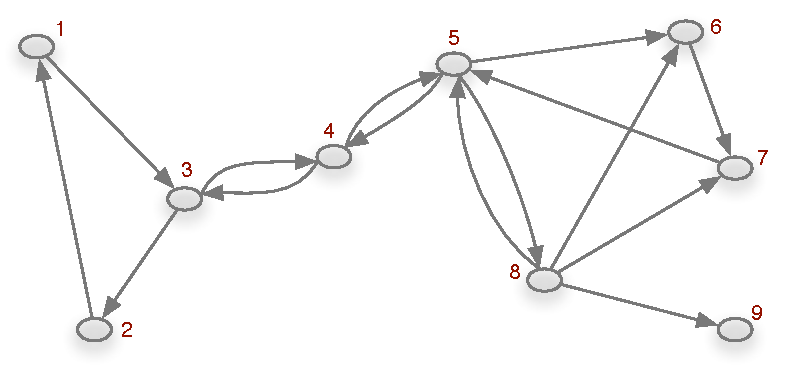
\includegraphics{DiGraph-Centrality}
\caption{A directed network for the demonstration of different centrality measures.}
\label{fig:example_net}
\end{center}
\end{figure}
%

\paragraph{Degree\color{Cayenne}{.}}
The simplest centrality measure is the degree $k$ of a node, which is the number of its neighbors.
In directed network, we distinguish between in-degree $k^-$ and out-degree $k^+$.
The degree follows immediately from the adjacency matrix, i.e.
\[
k_i ^- = \sum _j a_{ji} \quad \text{and} \quad k_i ^+ = \sum _j a_{ij}
\]
is the in- and out-degree of node $i$, respectively.
In weighted networks, the degree is computed in the same way and is called in-weight and out-weight of a node.

The degree centrality is used in a huge variety of applications.
One of its most important applications is to measure the heterogeneity of network connections, i.e. the existence of hubs in the network.
Hubs are nodes with a degree much larger than the rest of the system.
The heterogeneity of networks can be measured in terms of degree distributions (see section xx).


\paragraph{Closeness\color{Cayenne}{.}} 
The closeness of a node is the reciprocal average distance to all other nodes in the network.
It can be normalized, so that the closeness is $1$, if all other nodes are reachable within one step and $0$ in the limit of infinite distances to all other nodes.
The closeness of a node $i$ in a network of size $N$ is defined as follows:
\begin{equation}\label{eq:closeness}
c(i)=N-1 \sum _j \frac{1}{ d_{ij}}
\end{equation}
where $d_{ij}$ is the distance between nodes $i$ and $j$.
It should be noted that the distance between two nodes is defined to be infinite, if the underlying network is not connected.
In this case, the corresponding terms $1/\infty $ do not make contributions in equation \eqref{eq:closeness}.

The closeness centrality is capable to identify nodes with short average pathways to other parts of the network.
Identifying high closeness nodes is therefore reasonable for network navigation.
This holds in particular, if the exact route to the destination is unknown, because nodes with high closeness are probable to reach many destinations quickly.

\paragraph{Betweenness\color{Cayenne}{.}}
In order to identify nodes that act as bridges between two subgraphs, the measure of betweenness was developed.
In figure \ref{fig:example_net}, node $5$ plays such a role.
It is characteristic for these nodes to contain a relatively large number of shortest paths that have to cross them.
Therefore, betweenness of a node $i$ is defined as
\begin{equation}\label{eq:betweenness}
b(i)=\sum _{s\neq i \neq t} \frac{\sigma _{st}(i)}{\sigma _{st}}
\end{equation}
where $\sigma $ is .

Note that bridge nodes might look inconspicuous in the first place, e.g. they could have only two links.
Nevertheless, they play an important role for the division of networks into smaller pieces.
Betweenness centrality has been proven useful in order to divide networks into smaller components.
Therefore, nodes of high betweenness are removed from the network, so that the system disintegrates into smaller subgraphs \cite{xx}.


\paragraph{Eigenvector centrality\color{Cayenne}{.}}
The idea of eigenvector centrality can be easily realized by considering Markov chains as in section \ref{sec:network_matrices}.



\paragraph{Range\color{Cayenne}{.}}





\subsection{Implementation}

\subsection{From random mixing to developed structure}


\end{document}
